\textbf{See the instruction for questions \inteval{\value{question}+1} to \inteval{\value{question}+3}.}

\begin{center}
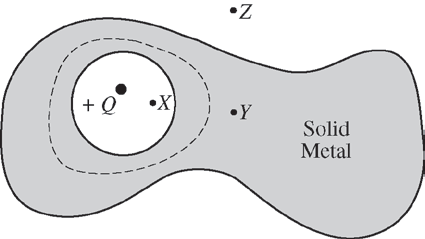
\includegraphics[scale=0.5]{images/img-003-006.png}
\end{center}

A charge $+Q$ is inside a hollow region in an electrically neutral piece of solid metal, as shown above. The dashed line represents a Gaussian surface within the metal that completely encloses the hollow region.

% Multiple Choice Question 8
\begin{questions}\setcounter{question}{7}\question
At which of the three labeled points is the electric field equal to zero?

\begin{oneparchoices}
\choice $X$ only
\choice $Y$ only
\choice $X$ and $Z$ only
\choice $Y$ and $Z$ only
\choice $X, Y$, and $Z$
\end{oneparchoices}\end{questions}

% Multiple Choice Question 9
\begin{questions}\setcounter{question}{8}\question
What is the net electric flux through the Gaussian surface?

\begin{choices}
\choice $-Q / \epsilon_{0}$
\choice Zero
\choice $+Q / \epsilon_{0}$
\choice $+2 Q / \epsilon_{0}$
\choice It cannot be determined without knowing the exact shape of the Gaussian surface.
\end{choices}\end{questions}

% Multiple Choice Question 10
\begin{questions}\setcounter{question}{9}\question
Which of the following correctly relates the electric potentials $V$ at points $X$, $Y$, and $Z$ ?

\begin{choices}
\choice $V_{X}<V_{Y}<V_{Z}$
\choice $V_{Y}<V_{X}<V_{Z} $
\choice $V_{Y}<V_{Z}<V_{X}$
\choice $V_{Z}<V_{X}<V_{Y}$
\choice $V_{Z}<V_{Y}<V_{X}$
\end{choices}\end{questions}

